\documentclass{article}
\usepackage{color,graphicx}
\usepackage{natbib}
\bibliographystyle{plainnat}
\usepackage[utf8]{inputenc}
\usepackage[swedish]{babel}


\author{Henrik Andersson}
\title{Probabilistisk våghöjdsprognos}

\begin{document}
\maketitle
    
\begin{abstract}
Våghöjd, risk \ldots
\end{abstract}

\section{Introdukton}

\citep{deo01}

\section{Metod}

Dropout är en populär metod för regularising av neurala nätverk. Dropout fungerar genom att ignorera signaler från slumpmässigt utvalda neuroner. Detta gör att modellen inte kan förlita sig på enskilda passager genom nätverket utan tvingas att hitta nya vägar och på så vis generalisera bättre.

Den typiska användingen av Dropout är att det endast är aktiv under träning av modellen och när modellen används för prediktion så är Dropout inte aktivt och modellen predikterar på så vis samma resultat varje gång med samma indata, dvs. en deterministisk modell.

\subsection{Data}

Observationer av våghöjd, riktning och period ~(Fig.~\ref{fig:data-test}) från SMHIs arkiv av öppna data från \citet{smhi}.

\begin{figure}
    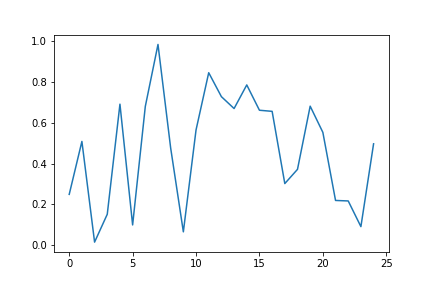
\includegraphics{fig/test}
    \caption{Test figur}
    \label{fig:data-test}
\end{figure}

\section{Resultat}

\section{Diskussion}


\bibliography{waves}




\end{document}